\documentclass[letterpaper,10pt]{article}
\usepackage[utf8]{inputenc}
\usepackage[spanish,mexico]{babel}
\usepackage{amsmath}
\usepackage{amsfonts}
\usepackage{amssymb}
\usepackage{enumerate}
\usepackage{float}
\usepackage{indentfirst}
\usepackage{graphicx}
\usepackage{url}
\usepackage{multicol}
\usepackage{geometry}
\usepackage{fullpage}
\usepackage{xcolor}
\usepackage{geometry}
\usepackage{algorithmic}
\usepackage{algorithm}
\usepackage{verbatim}
\usepackage[hidelinks]{hyperref}
\usepackage{subfigure}
\usepackage[hypcap=false]{caption}
\usepackage{tikz}
%\usetikzlibrary{shapes}
\usetikzlibrary{arrows,automata}

\tikzset{
    %Define standard arrow tip
    >=stealth',
    % Define arrow style
    pil/.style={
           ->,
           thick,}
}

\def\checkmark{\tikz\fill[scale=0.4](0,.35) -- (.25,0) -- (1,.7) -- (.25,.15) -- cycle;}

\begin{document}

\thispagestyle{empty}
 	
\begin{minipage}[t]{0.6\textwidth}

{\LARGE \textbf{INF152} Estructuras Discretas - Tarea 2}

{\large \textbf{Profesores}: Claudio Lobos, Jorge Díaz Sebastián Gallardo, María Paz Vergara y Miguel Guevara.}\\
{\small \textbf{Ayudantes}: Valentina Aróstica, Bryan González, Sofía Mañana, Sofía Riquelme, Carla Herrera, Álvaro Gaete, Constanza Alvarado, Maciel Ripetti, Maureen Gavilán, Ignacio Jorquera, Fernanda Avendaño y Luis González.} 

Universidad T\'ecnica Federico Santa Mar\'{\i}a

Departamento de Inform\'atica -- SJ - CC 



\end{minipage}
\hfill



\vspace{0.3cm}


\begin{center}
    \huge Tarea 2
\end{center}

\section{Reglas generales}
\begin{itemize}
    
    \item Para resolver cada pregunta, debe hacer uso de los contenidos, algoritmos y métodos aprendidos en el curso. Si su respuesta final es correcta, pero se ha utilizado un método distinto al enseñado en clases no se asignará puntaje. Ídem si entrega resultados sin desarrollo.
    
    \item La tarea debe realizarse en grupos de hasta 3 integrantes \textbf{\large DEL MISMO PARALELO}. Esta vez no habrán excepciones.
    
    \item Se descontará 5 puntos por warnings en el \texttt{.tex} (Excepto los warnings azules de Overleaf \textit{Underfull \textbackslash hbox (badness 10000)}, estos no tendrán descuentos).
    
    \item Si su proyecto \texttt{.tex} \textbf{no} compila tendrá 100 puntos de descuento sin opción a recorrección, inclusive si existe un \texttt{.pdf} con el desarrollo de la tarea.
        
    \item Tiene hasta las 23:59 hrs del día \textbf{9 de mayo} para entregar esta tarea vía Aula.
    
    \item No inserte su desarrollo en fotografías. Debe estar todo desarrollado en \LaTeX.
    
    \item Se restarán 10 puntos de su nota sucesivamente por cada hora de atraso.
    
    \subsection{Entrega}
     \item Sólo un integrante del grupo debe realizar la entrega.
     
     \item Se debe entregar un solo archivo \texttt{.zip} el cual debe contener:
     \begin{enumerate}
         \item El o los archivos \texttt{.tex} para compilar su tarea.
         \item Las imágenes adjuntas que permiten compilar el enunciado
         \item Un archivo \texttt{README.txt} que contenga los nombres de los integrantes del grupo, y sus roles.
     \end{enumerate}
     \item El archivo \texttt{.zip} debe tener como nombre: \texttt{nombre\_apellido.zip}, donde el nombre es el de el estudiante que hace la entrega.
     \item No es necesario incluir el \texttt{.pdf} en el \texttt{.zip}
    

    
\end{itemize}
\newpage
\section{Aprendiendo Pseudocodigo en latex}
\begin{enumerate}
    \item Resuelva el siguiente desafío programando en pseudocódigo. La solución debe escribirse en \LaTeX, usando los paquetes \textit{algorithmic} y \textit{algorithm} (los cuales ya están inluidos en este \texttt{.tex}).

Se da un \textcolor{blue}{String} $line$ conteniendo una lista de enteros, separados por uno o más espacios. Dado un int givenNumber, retornar el menor entero en line que sea estrictamente mayor que givenNumber. Retornar -1 si no existe tal número en line. [25 pts].
\vspace{0.5cm}

\textbf{Método:}
\begin{center}
    \textcolor{blue}{int} getLeast(\textcolor{blue}{String} line, \textcolor{blue}{int} givenNumber)
\end{center}

\textbf{Ejemplos:}
\vspace{0.5cm}

\begin{enumerate}
    \item[a)] \texttt{line = "1 2 3 4 5", givenNumber = 2}\\ Retorna: 3\\ 3 es el número más pequeño estrictamente mayor que 2.
    \item[b)] \texttt{line = "120 450 780", givenNumber = 1000}\\Retorna: -1\\No hay números estrictamente mayores que 1000.
    \item[c)] \texttt{line = "45 253 645 400 676 567", givenNumber = 1\\
Retorna: 45}
    \item[d)] \texttt{line = "45 253 645 400 676 567", givenNumber = 400}\\
Retorna: 567
    \item[e)] \texttt{line = "568 769 436 432 457 563 567 311 34 3 2 9", givenNumber = 460}\\
Retorna: 563
\end{enumerate}

\vspace{0.5cm}



%%%%%%%%%%%%%%%%%%%%%%%%%%%%%%%%%%%%%%%%%%%%%%%
Aquí tiene un pseudocódigo de ejemplo, que puede utilizar como plantilla para su solución:
%%%%%%%%%%%%%%%%%%%%%%%%%%%%%%%%%%%%%%%%%%%%%%%

\begin{center}
\begin{minipage}{0.6\textwidth}
\begin{algorithm}[H] %environment; permite texto flotante así no me salta de esta página a otra.
\begin{algorithmic}[1]%enumera las lineas de código de uno en uno; {algorithmic} 
%%%%%%%%%%%%%%%%%%%%%%%%%%%%%%%%%%%%%%%%%%%%%%%%%%%%%%%%%%%%%%%
%           AQUÍ EMPIEZA EL CÓDIGO DEL ALGORITMO:
%%%%%%%%%%%%%%%%%%%%%%%%%%%%%%%%%%%%%%%%%%%%%%%%%%%%%%%%%%%%%%%

\STATE{\textbf{Method} String nombreFuncion(String text)}
\STATE{  \textit{Empiece a programar aquí }}
\STATE{hola mundo}
\STATE{\textbf{string} variable $\leftarrow$ ''hola''}
\FOR{i in lista}
    \STATE{haz algo}
\ENDFOR
\WHILE{True}
    \PRINT{Hola}
\ENDWHILE


%%%%%%%%%%%%%%%%%%%%%%%%%%%%%%%%%%%%%%%%%%%%%%%%%%%%%%%%%%%%%%%
%           AQUÍ TERMINA EL CÓDIGO DEL ALGORITMO.
%%%%%%%%%%%%%%%%%%%%%%%%%%%%%%%%%%%%%%%%%%%%%%%%%%%%%%%%%%%%%%%
\end{algorithmic}
\caption{Titulo del algoritmo} %titulo
\label{alg:oculto} %etiqueta para referenciar algoritmo en doc.
\end{algorithm}
\end{minipage}
\end{center}

\textbf{Solución:}

\begin{center}
\begin{minipage}{0.9\textwidth}
\begin{algorithm}[H]
\begin{algorithmic}[1]

\STATE{\textbf{Method} int getLeast(String line, int givenNumber)}
\STATE{\textbf{int} x $\leftarrow$ 0}
\STATE{\textbf{int} y $\leftarrow$ 0}
\STATE{\textbf{int} lista $\leftarrow$ list() }
\FOR{item in line}
    \STATE{y $\leftarrow$ y+1}
    \STATE{\textbf{if} item \textbf{equals} ' ' \textbf{do}}
    \STATE{\hskip1.0em lista.append( stringToInt(line[x:y]) )}
    \STATE{\hskip1.0em x $\leftarrow$ y}
    \STATE{\textbf{end if}}
\ENDFOR
\STATE{\textbf{int} maxValue $\leftarrow$ 0}
\FOR{elemento1 in lista}
    \STATE{\textbf{if} elemento1 $ >$ maxValue \textbf{do}}
    \STATE{\hskip1.0em maxValue $\leftarrow$ elemento1}
    \STATE{\textbf{end if}}
\ENDFOR
\STATE{\textbf{if} maxValue $\leqslant$ givenNumber \textbf{do}}
\STATE{\hskip1.0em \textbf{return} -1}
\STATE{\textbf{end if}}
\FOR{elemento2 in lista}
    \STATE{\textbf{if} elemento2 $ >$ givenNumber \textbf{and} elemento2 $ < $ maxValue \textbf{do}}
    \STATE{\hskip1.0em maxValue $\leftarrow$ elemento2}
    \STATE{\textbf{endif}}
\ENDFOR
\STATE{\textbf{return} maxValue}
\STATE{\textit{// list() puede ser reemplazado por lista[], pero debe ser una estructura iterable}}
\STATE{\textit{// se asume la existencia de una funcion stringToInt() que transforme strings a enteros}}
\STATE{\textit{// se asume la existencia de un metodo append() que agrege elementos a lista}}

\end{algorithmic}
\caption{Find the minimum value larger than the parameter} %titulo
\label{solucion1} %etiqueta para referenciar algoritmo en doc.
\end{algorithm}
\end{minipage}
\end{center}


\end{enumerate}

\newpage
\section{Preguntas de Grafos y Árboles}
\begin{enumerate}
	\item Considere los siguientes grafos, dos de ellos representados en tablas de adyacencia, y conteste las preguntas relacionadas.\\
\begin{minipage}[b]{.25\textwidth}
\centering
\begin{tabular}{|l|llllll|}
\hline
&n&m&l&o&p&q\\
\hline
n & 0 & 0 & 1 & 1 & 1 & 0\\
m & 0 & 0 & 1 & 0 & 0 & 0\\
l & 1 & 1 & 0 & 1 & 0 & 0\\
o & 1 & 0 & 1 & 0 & 1 & 0\\
p & 1 & 0 & 0 & 1 & 0 & 1\\
q & 0 & 0 & 0 & 0 & 1 & 0\\
\hline
\end{tabular}
\captionof{table}{Matriz de Adyacencia de Grafo 1}
\label{eyl}
\end{minipage}
\hfill
\begin{minipage}[b]{.4\textwidth}
	\centering
	\begin{tabular}{|l|llllllll|}
	\hline
	  & a & b & c & d & e & f & g & h\\
	\hline
	a & 0 & 1 & 0 & 0 & 1 & 0 & 0 & 0\\
	b & 1 & 0 & 1 & 1 & 0 & 0 & 1 & 0\\
	c & 0 & 1 & 0 & 1 & 0 & 0 & 0 & 0\\
	d & 0 & 1 & 1 & 0 & 1 & 0 & 0 & 1\\
	e & 1 & 0 & 0 & 1 & 0 & 1 & 1 & 0\\
	f & 0 & 0 & 0 & 0 & 1 & 0 & 1 & 0\\
	g & 0 & 1 & 0 & 0 & 1 & 1 & 0 & 1\\
	h & 0 & 0 & 0 & 1 & 0 & 0 & 1 & 0\\

	\hline
	\end{tabular}
	\captionof{table}{Matriz de Adyacencia de Grafo 2}
	\label{ahsdfhj}
	\end{minipage}
\hfill
\begin{minipage}[b]{0.2\textwidth}
\centering
\begin{tikzpicture}[auto, node distance=1.5 cm,semithick]
\tikzstyle{every state}=[draw,minimum size=0.6cm]%,text=black]
%estados
\node[state] (a) {$a$};
\node[state] (f) [right of=a] {$f$};
\node[state] (b) [below of=a] {$b$};
\node[state] (e) [right of=b] {$e$};
\node[state] (c) [below of=b] {$c$};
\node[state] (d) [right of=c] {$d$};
%conexiones de los estados
\path 	(a) 	edge				node {}(f)
				edge				node {}(e)
				edge				node {}(b)
		(b)		edge				node {}(e)
				edge				node {}(c)
		(c)		edge				node {}(e)
				edge				node {}(d);
\end{tikzpicture}
\captionof{figure}{Grafo 3.}
\label{fig:sub1}
\end{minipage}

\begin{enumerate}
\item Utilizando el paquete Tikz de \LaTeX, dibuje los Grafos 1 y 2 expresados como matriz de adyacencia en las Tablas 1 y 2. No se aceptarán imágenes \textit{(El package ya está incluido en el header)} [10 pts].

\textbf{Solución:}

\item Demuestre o refute la existencia de un circuito de Euler en el grafo 2. ¿Existe Camino de Euler? En caso de que exista, nombre uno. [15 pts].

\textbf{Solución:}

\item Demuestre o refute: Grafo \textbf{1} y Grafo \textbf{3} son isomorfos [20 pts]

\textbf{Solución:}


\end{enumerate}
\newpage
\item Los sistemas operativos de las computadoras modernas organizan las carpetas y los archivos usando una estructura de árbol. Una carpeta contiene otras carpetas y archivos. La figura \ref{fig:archivos} muestra el explorador de Windows con el despliegue de carpetas. La raíz se llama INF152.

\begin{center}
    \begin{figure}[H]
    \centering
        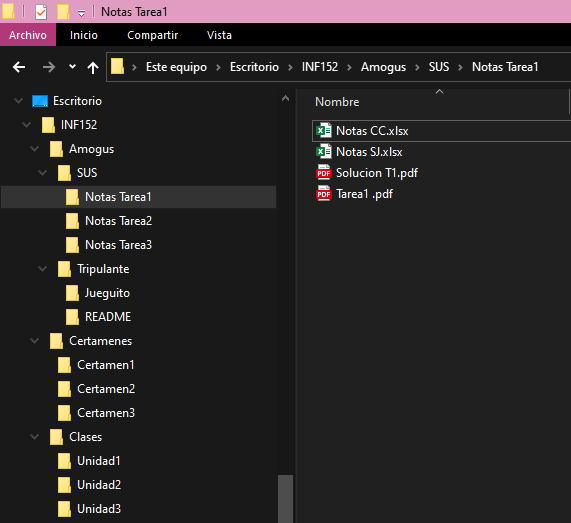
\includegraphics[scale=0.6]{inf152.png}
        \caption{Despliegue de explorador de archivos de Windows}
        \label{fig:archivos}
    \end{figure}
\end{center}

\begin{enumerate}
    \item Dibuje utilizando \LaTeX  el árbol que representa las carpetas de la Figura \ref{fig:archivos} [5 pts].\\
    \textbf{Solución:}
    \item Utilice los algoritmos de búsqueda en árboles para encontrar la solución del certamen 1 de la carpeta \textbf{Certamen1} y luego, realice los mismos pasos para encontrar un archivo dentro de la carpeta \textbf{Notas Tarea1}. ¿Puede determinar cuál búsqueda es más rápida en cada caso? Justifique.\\
    \textit{(Puede dibujar con Tikz el paso a paso en los grafos y marcar con colores las rutas de búsqueda. Otra forma es explicar con pseudocódigo o puede escribir un ruteo de los algoritmos. Lo importante es que explique formalmente cómo ejecuta los algoritmos.)} [25 pts].
    
    \textbf{Solución:}
\end{enumerate}


\end{enumerate}




\end{document}